\documentclass[11pt,compress,t,notes=noshow, aspectratio=169, xcolor=table]{beamer}

\usepackage{../../style/lmu-lecture}
% Defines macros and environments
\usepackage[]{graphicx}
\usepackage[]{color}
% maxwidth is the original width if it is less than linewidth
% otherwise use linewidth (to make sure the graphics do not exceed the margin)
\makeatletter
\def\maxwidth{ %
\ifdim\Gin@nat@width>\linewidth
\linewidth
\else
\Gin@nat@width
\fi
}
\makeatother
%\usepackage[fontsize=10.5pt]{scrextend}
\definecolor{ggred}{rgb}{0.973, 0.463, 0.427}
\definecolor{ggblue}{rgb}{0, 0.749, 0.769}
\definecolor{fgcolor}{rgb}{0.345, 0.345, 0.345}
\newcommand{\hlnum}[1]{\textcolor[rgb]{0.686,0.059,0.569}{#1}}%
\newcommand{\hlstr}[1]{\textcolor[rgb]{0.192,0.494,0.8}{#1}}%
\newcommand{\hlcom}[1]{\textcolor[rgb]{0.678,0.584,0.686}{\textit{#1}}}%
\newcommand{\hlopt}[1]{\textcolor[rgb]{0,0,0}{#1}}%
\newcommand{\hlstd}[1]{\textcolor[rgb]{0.345,0.345,0.345}{#1}}%
\newcommand{\hlkwa}[1]{\textcolor[rgb]{0.161,0.373,0.58}{\textbf{#1}}}%
\newcommand{\hlkwb}[1]{\textcolor[rgb]{0.69,0.353,0.396}{#1}}%
\newcommand{\hlkwc}[1]{\textcolor[rgb]{0.333,0.667,0.333}{#1}}%
\newcommand{\hlkwd}[1]{\textcolor[rgb]{0.737,0.353,0.396}{\textbf{#1}}}%
\newcommand{\predvar}{Var\left[\hat{f}(\xv)\right]}
\let\hlipl\hlkwb

\usepackage{pdfpages}
\usepackage{framed}
\makeatletter
\newenvironment{kframe}{%
\def\at@end@of@kframe{}%
\ifinner\ifhmode%
\def\at@end@of@kframe{\end{minipage}}%
\begin{minipage}{\columnwidth}%
\fi\fi%
\def\FrameCommand##1{\hskip\@totalleftmargin \hskip-\fboxsep
\colorbox{shadecolor}{##1}\hskip-\fboxsep
% There is no \\@totalrightmargin, so:
\hskip-\linewidth \hskip-\@totalleftmargin \hskip\columnwidth}%
\MakeFramed {\advance\hsize-\width
\@totalleftmargin\z@ \linewidth\hsize
\@setminipage}}%
{\par\unskip\endMakeFramed%
\at@end@of@kframe}
\makeatother

\definecolor{shadecolor}{rgb}{.97, .97, .97}
\definecolor{messagecolor}{rgb}{0, 0, 0}
\definecolor{warningcolor}{rgb}{1, 0, 1}
\definecolor{errorcolor}{rgb}{1, 0, 0}
\newenvironment{knitrout}{}{} % an empty environment to be redefined in TeX

\usepackage{alltt}
\newcommand{\SweaveOpts}[1]{}  % do not interfere with LaTeX
\newcommand{\SweaveInput}[1]{} % because they are not real TeX commands
\newcommand{\Sexpr}[1]{}       % will only be parsed by R

\usepackage[english]{babel}
\usepackage[utf8]{inputenc}

\usepackage[export]{adjustbox}
\usepackage{dsfont}
\usepackage{verbatim}
\usepackage{amsmath}
\usepackage{amsfonts}
\usepackage{bm}
\usepackage{csquotes}
\usepackage{multirow}
\usepackage{longtable}
\usepackage{booktabs}
\usepackage{enumerate}
\usepackage[absolute,overlay]{textpos}
\usepackage{psfrag}
\usepackage{algorithm}
\usepackage{algpseudocode}
\usepackage{eqnarray}
\usepackage{arydshln}
\usepackage{tabularx}
\usepackage{placeins}
\usepackage{tikz}
\usepackage{setspace}
\usepackage{colortbl}
\usepackage{mathtools}
\usepackage{wrapfig}
\usepackage{bm}
\usepackage[backend=biber]{biblatex}

\usetikzlibrary{tikzmark, shapes,arrows,automata,positioning,calc,chains,trees,  shadows, decorations.pathreplacing}
\tikzset{
%Define standard arrow tip
>=stealth',
%Define style for boxes
punkt/.style={
rectangle,
rounded corners,
draw=black, very thick,
text width=6.5em,
minimum height=2em,
text centered},
% Define arrow style
pil/.style={
->,
thick,
shorten <=2pt,
shorten >=2pt,}
}

\usepackage{subfig}

\usepackage{bbm}
%\newcommand\hmmax{0}
%\newcommand\bmmax{0}
% basic latex stuff
\newcommand{\pkg}[1]{{\fontseries{b}\selectfont #1}} %fontstyle for R packages
\newcommand{\lz}{\vspace{0.5cm}} %vertical space
\newcommand{\dlz}{\vspace{1cm}} %double vertical space
\newcommand{\oneliner}[1] % Oneliner for important statements
{\begin{block}{}\begin{center}\begin{Large}#1\end{Large}\end{center}\end{block}}

% Latexmath Notation
% math spaces
\ifdefined\N                                                                
\renewcommand{\N}{\mathds{N}} % N, naturals
\else \newcommand{\N}{\mathds{N}} \fi 
\newcommand{\Z}{\mathds{Z}} % Z, integers
\newcommand{\Q}{\mathds{Q}} % Q, rationals
\newcommand{\R}{\mathds{R}} % R, reals
\ifdefined\C 
  \renewcommand{\C}{\mathds{C}} % C, complex
\else \newcommand{\C}{\mathds{C}} \fi
\newcommand{\continuous}{\mathcal{C}} % C, space of continuous functions
\newcommand{\M}{\mathcal{M}} % machine numbers
\newcommand{\epsm}{\epsilon_m} % maximum error

% counting / finite sets
\newcommand{\setzo}{\{0, 1\}} % set 0, 1
\newcommand{\setmp}{\{-1, +1\}} % set -1, 1
\newcommand{\unitint}{[0, 1]} % unit interval

% basic math stuff
\newcommand{\xt}{\tilde x} % x tilde
\newcommand{\argmax}{\operatorname{arg\,max}} % argmax
\newcommand{\argmin}{\operatorname{arg\,min}} % argmin
\newcommand{\argminlim}{\mathop{\mathrm{arg\,min}}\limits} % argmax with limits
\newcommand{\argmaxlim}{\mathop{\mathrm{arg\,max}}\limits} % argmin with limits  
\newcommand{\sign}{\operatorname{sign}} % sign, signum
\newcommand{\I}{\mathbb{I}} % I, indicator
\newcommand{\order}{\mathcal{O}} % O, order
\newcommand{\pd}[2]{\frac{\partial{#1}}{\partial #2}} % partial derivative
\newcommand{\floorlr}[1]{\left\lfloor #1 \right\rfloor} % floor
\newcommand{\ceillr}[1]{\left\lceil #1 \right\rceil} % ceiling

% sums and products
\newcommand{\sumin}{\sum\limits_{i=1}^n} % summation from i=1 to n
\newcommand{\sumim}{\sum\limits_{i=1}^m} % summation from i=1 to m
\newcommand{\sumjn}{\sum\limits_{j=1}^n} % summation from j=1 to p
\newcommand{\sumjp}{\sum\limits_{j=1}^p} % summation from j=1 to p
\newcommand{\sumik}{\sum\limits_{i=1}^k} % summation from i=1 to k
\newcommand{\sumkg}{\sum\limits_{k=1}^g} % summation from k=1 to g
\newcommand{\sumjg}{\sum\limits_{j=1}^g} % summation from j=1 to g
\newcommand{\meanin}{\frac{1}{n} \sum\limits_{i=1}^n} % mean from i=1 to n
\newcommand{\meanim}{\frac{1}{m} \sum\limits_{i=1}^m} % mean from i=1 to n
\newcommand{\meankg}{\frac{1}{g} \sum\limits_{k=1}^g} % mean from k=1 to g
\newcommand{\prodin}{\prod\limits_{i=1}^n} % product from i=1 to n
\newcommand{\prodkg}{\prod\limits_{k=1}^g} % product from k=1 to g
\newcommand{\prodjp}{\prod\limits_{j=1}^p} % product from j=1 to p

% linear algebra
\newcommand{\one}{\boldsymbol{1}} % 1, unitvector
\newcommand{\zero}{\mathbf{0}} % 0-vector
\newcommand{\id}{\boldsymbol{I}} % I, identity
\newcommand{\diag}{\operatorname{diag}} % diag, diagonal
\newcommand{\trace}{\operatorname{tr}} % tr, trace
\newcommand{\spn}{\operatorname{span}} % span
\newcommand{\scp}[2]{\left\langle #1, #2 \right\rangle} % <.,.>, scalarproduct
\newcommand{\mat}[1]{\begin{pmatrix} #1 \end{pmatrix}} % short pmatrix command
\newcommand{\Amat}{\mathbf{A}} % matrix A
\newcommand{\Deltab}{\mathbf{\Delta}} % error term for vectors

% basic probability + stats
\renewcommand{\P}{\mathds{P}} % P, probability
\newcommand{\E}{\mathds{E}} % E, expectation
\newcommand{\var}{\mathsf{Var}} % Var, variance
\newcommand{\cov}{\mathsf{Cov}} % Cov, covariance
\newcommand{\corr}{\mathsf{Corr}} % Corr, correlation
\newcommand{\normal}{\mathcal{N}} % N of the normal distribution
\newcommand{\iid}{\overset{i.i.d}{\sim}} % dist with i.i.d superscript
\newcommand{\distas}[1]{\overset{#1}{\sim}} % ... is distributed as ...

% machine learning
\newcommand{\Xspace}{\mathcal{X}} % X, input space
\newcommand{\Yspace}{\mathcal{Y}} % Y, output space
\newcommand{\nset}{\{1, \ldots, n\}} % set from 1 to n
\newcommand{\pset}{\{1, \ldots, p\}} % set from 1 to p
\newcommand{\gset}{\{1, \ldots, g\}} % set from 1 to g
\newcommand{\Pxy}{\mathbb{P}_{xy}} % P_xy
\newcommand{\Exy}{\mathbb{E}_{xy}} % E_xy: Expectation over random variables xy
\newcommand{\xv}{\mathbf{x}} % vector x (bold)
\newcommand{\xtil}{\tilde{\mathbf{x}}} % vector x-tilde (bold)
\newcommand{\yv}{\mathbf{y}} % vector y (bold)
\newcommand{\xy}{(\xv, y)} % observation (x, y)
\newcommand{\xvec}{\left(x_1, \ldots, x_p\right)^\top} % (x1, ..., xp) 
\newcommand{\Xmat}{\mathbf{X}} % Design matrix
\newcommand{\allDatasets}{\mathds{D}} % The set of all datasets
\newcommand{\allDatasetsn}{\mathds{D}_n}  % The set of all datasets of size n 
\newcommand{\D}{\mathcal{D}} % D, data
\newcommand{\Dn}{\D_n} % D_n, data of size n
\newcommand{\Dtrain}{\mathcal{D}_{\text{train}}} % D_train, training set
\newcommand{\Dtest}{\mathcal{D}_{\text{test}}} % D_test, test set
\newcommand{\xyi}[1][i]{\left(\xv^{(#1)}, y^{(#1)}\right)} % (x^i, y^i), i-th observation
\newcommand{\Dset}{\left( \xyi[1], \ldots, \xyi[n]\right)} % {(x1,y1)), ..., (xn,yn)}, data
\newcommand{\defAllDatasetsn}{(\Xspace \times \Yspace)^n} % Def. of the set of all datasets of size n 
\newcommand{\defAllDatasets}{\bigcup_{n \in \N}(\Xspace \times \Yspace)^n} % Def. of the set of all datasets 
\newcommand{\xdat}{\left\{ \xv^{(1)}, \ldots, \xv^{(n)}\right\}} % {x1, ..., xn}, input data
\newcommand{\ydat}{\left\{ \yv^{(1)}, \ldots, \yv^{(n)}\right\}} % {y1, ..., yn}, input data
\newcommand{\yvec}{\left(y^{(1)}, \hdots, y^{(n)}\right)^\top} % (y1, ..., yn), vector of outcomes
\renewcommand{\xi}[1][i]{\xv^{(#1)}} % x^i, i-th observed value of x
\newcommand{\yi}[1][i]{y^{(#1)}} % y^i, i-th observed value of y 
\newcommand{\xivec}{\left(x^{(i)}_1, \ldots, x^{(i)}_p\right)^\top} % (x1^i, ..., xp^i), i-th observation vector
\newcommand{\xj}{\xv_j} % x_j, j-th feature
\newcommand{\xjvec}{\left(x^{(1)}_j, \ldots, x^{(n)}_j\right)^\top} % (x^1_j, ..., x^n_j), j-th feature vector
\newcommand{\phiv}{\mathbf{\phi}} % Basis transformation function phi
\newcommand{\phixi}{\mathbf{\phi}^{(i)}} % Basis transformation of xi: phi^i := phi(xi)

%%%%%% ml - models general
\newcommand{\lamv}{\bm{\lambda}} % lambda vector, hyperconfiguration vector
\newcommand{\Lam}{\bm{\Lambda}}	 % Lambda, space of all hpos
% Inducer / Inducing algorithm
\newcommand{\preimageInducer}{\left(\defAllDatasets\right)\times\Lam} % Set of all datasets times the hyperparameter space
\newcommand{\preimageInducerShort}{\allDatasets\times\Lam} % Set of all datasets times the hyperparameter space
% Inducer / Inducing algorithm
\newcommand{\ind}{\mathcal{I}} % Inducer, inducing algorithm, learning algorithm 

% continuous prediction function f
\newcommand{\ftrue}{f_{\text{true}}}  % True underlying function (if a statistical model is assumed)
\newcommand{\ftruex}{\ftrue(\xv)} % True underlying function (if a statistical model is assumed)
\newcommand{\fx}{f(\xv)} % f(x), continuous prediction function
\newcommand{\fdomains}{f: \Xspace \rightarrow \R^g} % f with domain and co-domain
\newcommand{\Hspace}{\mathcal{H}} % hypothesis space where f is from
\newcommand{\fbayes}{f^{\ast}} % Bayes-optimal model
\newcommand{\fxbayes}{f^{\ast}(\xv)} % Bayes-optimal model
\newcommand{\fkx}[1][k]{f_{#1}(\xv)} % f_j(x), discriminant component function
\newcommand{\fh}{\hat{f}} % f hat, estimated prediction function
\newcommand{\fxh}{\fh(\xv)} % fhat(x)
\newcommand{\fxt}{f(\xv ~|~ \thetab)} % f(x | theta)
\newcommand{\fxi}{f\left(\xv^{(i)}\right)} % f(x^(i))
\newcommand{\fxih}{\hat{f}\left(\xv^{(i)}\right)} % f(x^(i))
\newcommand{\fxit}{f\left(\xv^{(i)} ~|~ \thetab\right)} % f(x^(i) | theta)
\newcommand{\fhD}{\fh_{\D}} % fhat_D, estimate of f based on D
\newcommand{\fhDtrain}{\fh_{\Dtrain}} % fhat_Dtrain, estimate of f based on D
\newcommand{\fhDnlam}{\fh_{\Dn, \lamv}} %model learned on Dn with hp lambda
\newcommand{\fhDlam}{\fh_{\D, \lamv}} %model learned on D with hp lambda
\newcommand{\fhDnlams}{\fh_{\Dn, \lamv^\ast}} %model learned on Dn with optimal hp lambda 
\newcommand{\fhDlams}{\fh_{\D, \lamv^\ast}} %model learned on D with optimal hp lambda 

% discrete prediction function h
\newcommand{\hx}{h(\xv)} % h(x), discrete prediction function
\newcommand{\hh}{\hat{h}} % h hat
\newcommand{\hxh}{\hat{h}(\xv)} % hhat(x)
\newcommand{\hxt}{h(\xv | \thetab)} % h(x | theta)
\newcommand{\hxi}{h\left(\xi\right)} % h(x^(i))
\newcommand{\hxit}{h\left(\xi ~|~ \thetab\right)} % h(x^(i) | theta)
\newcommand{\hbayes}{h^{\ast}} % Bayes-optimal classification model
\newcommand{\hxbayes}{h^{\ast}(\xv)} % Bayes-optimal classification model

% yhat
\newcommand{\yh}{\hat{y}} % yhat for prediction of target
\newcommand{\yih}{\hat{y}^{(i)}} % yhat^(i) for prediction of ith targiet
\newcommand{\resi}{\yi- \yih}

% theta
\newcommand{\thetah}{\hat{\theta}} % theta hat
\newcommand{\thetab}{\bm{\theta}} % theta vector
\newcommand{\thetabh}{\bm{\hat\theta}} % theta vector hat
\newcommand{\thetat}[1][t]{\thetab^{[#1]}} % theta^[t] in optimization
\newcommand{\thetatn}[1][t]{\thetab^{[#1 +1]}} % theta^[t+1] in optimization
\newcommand{\thetahDnlam}{\thetabh_{\Dn, \lamv}} %theta learned on Dn with hp lambda
\newcommand{\thetahDlam}{\thetabh_{\D, \lamv}} %theta learned on D with hp lambda
\newcommand{\mint}{\min_{\thetab \in \Theta}} % min problem theta
\newcommand{\argmint}{\argmin_{\thetab \in \Theta}} % argmin theta

% densities + probabilities
% pdf of x 
\newcommand{\pdf}{p} % p
\newcommand{\pdfx}{p(\xv)} % p(x)
\newcommand{\pixt}{\pi(\xv~|~ \thetab)} % pi(x|theta), pdf of x given theta
\newcommand{\pixit}[1][i]{\pi\left(\xi[#1] ~|~ \thetab\right)} % pi(x^i|theta), pdf of x given theta
\newcommand{\pixii}[1][i]{\pi\left(\xi[#1]\right)} % pi(x^i), pdf of i-th x 

% pdf of (x, y)
\newcommand{\pdfxy}{p(\xv,y)} % p(x, y)
\newcommand{\pdfxyt}{p(\xv, y ~|~ \thetab)} % p(x, y | theta)
\newcommand{\pdfxyit}{p\left(\xi, \yi ~|~ \thetab\right)} % p(x^(i), y^(i) | theta)

% pdf of x given y
\newcommand{\pdfxyk}[1][k]{p(\xv | y= #1)} % p(x | y = k)
\newcommand{\lpdfxyk}[1][k]{\log p(\xv | y= #1)} % log p(x | y = k)
\newcommand{\pdfxiyk}[1][k]{p\left(\xi | y= #1 \right)} % p(x^i | y = k)

% prior probabilities
\newcommand{\pik}[1][k]{\pi_{#1}} % pi_k, prior
\newcommand{\lpik}[1][k]{\log \pi_{#1}} % log pi_k, log of the prior
\newcommand{\pit}{\pi(\thetab)} % Prior probability of parameter theta

% posterior probabilities
\newcommand{\post}{\P(y = 1 ~|~ \xv)} % P(y = 1 | x), post. prob for y=1
\newcommand{\postk}[1][k]{\P(y = #1 ~|~ \xv)} % P(y = k | y), post. prob for y=k
\newcommand{\pidomains}{\pi: \Xspace \rightarrow \unitint} % pi with domain and co-domain
\newcommand{\pibayes}{\pi^{\ast}} % Bayes-optimal classification model
\newcommand{\pixbayes}{\pi^{\ast}(\xv)} % Bayes-optimal classification model
\newcommand{\pix}{\pi(\xv)} % pi(x), P(y = 1 | x)
\newcommand{\piv}{\bm{\pi}} % pi, bold, as vector
\newcommand{\pikx}[1][k]{\pi_{#1}(\xv)} % pi_k(x), P(y = k | x)
\newcommand{\pikxt}[1][k]{\pi_{#1}(\xv ~|~ \thetab)} % pi_k(x | theta), P(y = k | x, theta)
\newcommand{\pixh}{\hat \pi(\xv)} % pi(x) hat, P(y = 1 | x) hat
\newcommand{\pikxh}[1][k]{\hat \pi_{#1}(\xv)} % pi_k(x) hat, P(y = k | x) hat
\newcommand{\pixih}{\hat \pi(\xi)} % pi(x^(i)) with hat
\newcommand{\pikxih}[1][k]{\hat \pi_{#1}(\xi)} % pi_k(x^(i)) with hat
\newcommand{\pdfygxt}{p(y ~|~\xv, \thetab)} % p(y | x, theta)
\newcommand{\pdfyigxit}{p\left(\yi ~|~\xi, \thetab\right)} % p(y^i |x^i, theta)
\newcommand{\lpdfygxt}{\log \pdfygxt } % log p(y | x, theta)
\newcommand{\lpdfyigxit}{\log \pdfyigxit} % log p(y^i |x^i, theta)

% probababilistic
\newcommand{\bayesrulek}[1][k]{\frac{\P(\xv | y= #1) \P(y= #1)}{\P(\xv)}} % Bayes rule
\newcommand{\muk}{\bm{\mu_k}} % mean vector of class-k Gaussian (discr analysis) 

% residual and margin
\newcommand{\eps}{\epsilon} % residual, stochastic
\newcommand{\epsi}{\epsilon^{(i)}} % epsilon^i, residual, stochastic
\newcommand{\epsh}{\hat{\epsilon}} % residual, estimated
\newcommand{\yf}{y \fx} % y f(x), margin
\newcommand{\yfi}{\yi \fxi} % y^i f(x^i), margin
\newcommand{\Sigmah}{\hat \Sigma} % estimated covariance matrix
\newcommand{\Sigmahj}{\hat \Sigma_j} % estimated covariance matrix for the j-th class

% ml - loss, risk, likelihood
\newcommand{\Lyf}{L\left(y, f\right)} % L(y, f), loss function
\newcommand{\Lypi}{L\left(y, \pi\right)} % L(y, pi), loss function
\newcommand{\Lxy}{L\left(y, \fx\right)} % L(y, f(x)), loss function
\newcommand{\Lxyi}{L\left(\yi, \fxi\right)} % loss of observation
\newcommand{\Lxyt}{L\left(y, \fxt\right)} % loss with f parameterized
\newcommand{\Lxyit}{L\left(\yi, \fxit\right)} % loss of observation with f parameterized
\newcommand{\Lxym}{L\left(\yi, f\left(\bm{\tilde{x}}^{(i)} ~|~ \thetab\right)\right)} % loss of observation with f parameterized
\newcommand{\Lpixy}{L\left(y, \pix\right)} % loss in classification
\newcommand{\Lpiv}{L\left(y, \piv\right)} % loss in classification
\newcommand{\Lpixyi}{L\left(\yi, \pixii\right)} % loss of observation in classification
\newcommand{\Lpixyt}{L\left(y, \pixt\right)} % loss with pi parameterized
\newcommand{\Lpixyit}{L\left(\yi, \pixit\right)} % loss of observation with pi parameterized
\newcommand{\Lhxy}{L\left(y, \hx\right)} % L(y, h(x)), loss function on discrete classes
\newcommand{\Lr}{L\left(r\right)} % L(r), loss defined on residual (reg) / margin (classif)
\newcommand{\lone}{|y - \fx|} % L1 loss
\newcommand{\ltwo}{\left(y - \fx\right)^2} % L2 loss
\newcommand{\lbernoullimp}{\ln(1 + \exp(-y \cdot \fx))} % Bernoulli loss for -1, +1 encoding
\newcommand{\lbernoullizo}{- y \cdot \fx + \log(1 + \exp(\fx))} % Bernoulli loss for 0, 1 encoding
\newcommand{\lcrossent}{- y \log \left(\pix\right) - (1 - y) \log \left(1 - \pix\right)} % cross-entropy loss
\newcommand{\lbrier}{\left(\pix - y \right)^2} % Brier score
\newcommand{\risk}{\mathcal{R}} % R, risk
\newcommand{\riskbayes}{\mathcal{R}^\ast}
\newcommand{\riskf}{\risk(f)} % R(f), risk
\newcommand{\riskdef}{\E_{y|\xv}\left(\Lxy \right)} % risk def (expected loss)
\newcommand{\riskt}{\mathcal{R}(\thetab)} % R(theta), risk
\newcommand{\riske}{\mathcal{R}_{\text{emp}}} % R_emp, empirical risk w/o factor 1 / n
\newcommand{\riskeb}{\bar{\mathcal{R}}_{\text{emp}}} % R_emp, empirical risk w/ factor 1 / n
\newcommand{\riskef}{\riske(f)} % R_emp(f)
\newcommand{\risket}{\mathcal{R}_{\text{emp}}(\thetab)} % R_emp(theta)
\newcommand{\riskr}{\mathcal{R}_{\text{reg}}} % R_reg, regularized risk
\newcommand{\riskrt}{\mathcal{R}_{\text{reg}}(\thetab)} % R_reg(theta)
\newcommand{\riskrf}{\riskr(f)} % R_reg(f)
\newcommand{\riskrth}{\hat{\mathcal{R}}_{\text{reg}}(\thetab)} % hat R_reg(theta)
\newcommand{\risketh}{\hat{\mathcal{R}}_{\text{emp}}(\thetab)} % hat R_emp(theta)
\newcommand{\LL}{\mathcal{L}} % L, likelihood
\newcommand{\LLt}{\mathcal{L}(\thetab)} % L(theta), likelihood
\newcommand{\LLtx}{\mathcal{L}(\thetab | \xv)} % L(theta|x), likelihood
\newcommand{\logl}{\ell} % l, log-likelihood
\newcommand{\loglt}{\logl(\thetab)} % l(theta), log-likelihood
\newcommand{\logltx}{\logl(\thetab | \xv)} % l(theta|x), log-likelihood
\newcommand{\errtrain}{\text{err}_{\text{train}}} % training error
\newcommand{\errtest}{\text{err}_{\text{test}}} % test error
\newcommand{\errexp}{\overline{\text{err}_{\text{test}}}} % avg training error

% lm
\newcommand{\thx}{\thetab^\top \xv} % linear model
\newcommand{\olsest}{(\Xmat^\top \Xmat)^{-1} \Xmat^\top \yv} % OLS estimator in LM 

%%%%%% perturbed data
\usepackage{xifthen}
\newcommand{\pert}[3]{\ifthenelse{\equal{#2}{}}{\tilde{#1}}{\ifthenelse{\equal{#3}{}}{\tilde{#1}^{#2}}{\tilde{#1}^{#2|#3}}}}	% command to express that for #1 the subset #2 was perturbed given subset #3

%%%%%% marginalized functions
\newcommand{\fj}{f_j} % marginal function f_j, depending on feature j
\newcommand{\fnj}{f_{-j}} % marginal function f_{-j}, depending on all features but j
\newcommand{\fS}{f_S} % marginal function f_S depending on feature set S
\newcommand{\fnj}{f_{-S}} % marginal function f_{-S}, depending on all features but features in S
\newcommand{\fC}{f_C} % marginal function f_C depending on feature set C
\newcommand{\fhj}{\fh_j} % marginal function fh_j, depending on feature j
\newcommand{\fhnj}{\fh_{-j}} % marginal function fh_{-j}, depending on all features but j
\newcommand{\fhS}{\fh_S} % marginal function fh_S depending on feature set S
\newcommand{\fhnS}{\fh_{-S}} % marginal function fh_{-S}, depending on all features but features in S
\newcommand{\fhC}{\fh_C} % marginal function fh_C depending on feature set C
\newcommand{\XSmat}{\Xmat_S} % Design matrix subset
\newcommand{\XnSmat}{\Xmat__{-S}} % Design matrix subset without S
\newcommand{\XCmat}{\Xmat_C} % Design matrix subset
\newcommand{\Xnj}{\Xmat_{-j}} % Design matrix subset -j = {1, .., j-1, j+1, ..., p}

%%%%% Shapley values
\newcommand{\Scupj}{S \cup \{j\}} % coalition S but without player j
\newcommand{\Scupk}{S \cup \{k\}} % coalition S but without player k
\newcommand{\SsubP}{S \subseteq P} % coalition S subset of P
\newcommand{\SsubPnoj}{\SsubP \setminus \{j\}} % coalition S subset of P without player j
\newcommand{\SsubPnojk}{\SsubP \setminus \{j,k\}} % coalition S subset of P without player k
\newcommand{\phiij}{\hat{\phi}_j^{(i)}} % Shapley value for feature j and observation i

%%%%% LIME 
\newcommand{\Gspace}{\mathcal{G}} % Hypothesis space for surrogate model
\newcommand{\neigh}{\phi_{\xv}} % Proximity measure
\newcommand{\zv}{\mathbf{z}} % Sampled datapoints for surrogate
\newcommand{\Zspace}{\mathcal{Z}} % Space of sampled datapoints
\newcommand{\Gower}{d_G} % Gower distance


\newcommand{\indep}{\perp}
\newcommand{\Ind}{\mathcal{I}}

%new environments
\newenvironment{vbframe}  %frame with breaks and verbatim
{
\begin{frame}%[containsverbatim,allowframebreaks]
}
{
\end{frame}
}

% \newenvironment{vframe}  %frame with verbatim without breaks (to avoid numbering one slided frames)
% {
%  \begin{frame}[containsverbatim]
% }
% {
% \end{frame}
% }

\newenvironment{blocki}[1]   % itemize block
{
 \begin{block}{#1}\begin{itemize}
}
{
\end{itemize}\end{block}
}

\newenvironment{fragileframe}[2]{  %fragile frame with framebreaks
\begin{frame}[allowframebreaks, fragile, environment = fragileframe]
\frametitle{#1}
#2}
{\end{frame}}


\newcommand{\myframe}[2]{  %short for frame with framebreaks
\begin{frame}[allowframebreaks]
\frametitle{#1}
#2
\end{frame}}

\newcommand{\remark}[1]{
  \textbf{Remark:} #1
}


\newenvironment{deleteframe}
{
\begingroup
\usebackgroundtemplate{
\includegraphics[width=\paperwidth,height=\paperheight]{../style/color/red.png}}
 \begin{frame}
}
{
\end{frame}
\endgroup
}
\newenvironment{simplifyframe}
{
\begingroup
\usebackgroundtemplate{
\includegraphics[width=\paperwidth,height=\paperheight]{../style/color/yellow.png}}
 \begin{frame}
}
{
\end{frame}
\endgroup
}\newenvironment{draftframe}
{
\begingroup
\usebackgroundtemplate{
\includegraphics[width=\paperwidth,height=\paperheight]{../style/color/green.jpg}}
 \begin{frame}
}
{
\end{frame}
\endgroup
}
% https://tex.stackexchange.com/a/261480: textcolor that works in mathmode
\makeatletter
\renewcommand*{\@textcolor}[3]{%
  \protect\leavevmode
  \begingroup
    \color#1{#2}#3%
  \endgroup
}
\makeatother

% \makeatletter
% %\newcommand\notsotiny{\@setfontsize\notsotiny\@vipt\@viipt}
% \newcommand\notsotiny{\@setfontsize\notsotiny{6.31415}{7.1828}}
% \makeatother

\providecommand{\tightlist}{%
  \setlength{\itemsep}{0pt}\setlength{\parskip}{0pt}}

%\setbeamerfont{footnote}{size=\tiny}
\usepackage[hang,flushmargin]{footmisc}
\renewcommand*{\footnotelayout}{\tiny}
\renewcommand*{\thefootnote}{} %\fnsymbol{footnote}

% https://tex.stackexchange.com/questions/638616/beamer-frametitle-always-uppercase-for-text-but-not-for-href-or-url
\usepackage{textcase}

% https://stackoverflow.com/questions/377301/is-there-a-latex-command-to-make-text-all-lower-caps
%\usepackage[overload]{textcase}
%\setbeamertemplate{frametitle}{\MakeTextUppercase{\insertframetitle}}
%\setbeamertemplate{frametitle}{\expandafter\uppercase\expandafter\insertframetitle}

\setbeamertemplate{frametitle}{\MakeTextUppercase{\insertframetitle}}
\newcommand{\citebutton}[2]{%
\NoCaseChange{\resizebox{!}{9pt}{\protect\beamergotobutton{\href{#2}{#1}}}}%
}

%\setbeamertemplate{frametitle}{\expandafter\uppercase\expandafter\insertframetitle}
%\newcommand{\citebutton}[2]{%
%\href{#2}{\footnotesize\color{black!60}[#1]}
%\resizebox{!}{9pt}{\beamergotobutton{\lowercase{\href{#2}}{#1}}}% \MakeLowercase
%}
%\newcommand{\lit}[2]{\href{#2}{\footnotesize\color{black!60}[#1]}}

\newcommand{\lit}[2]{\href{#2}{\footnotesize\color{black!60}[#1]}}

\let\code=\texttt
\let\proglang=\textsf

\setkeys{Gin}{width=0.9\textwidth}

% https://tex.stackexchange.com/questions/30720/footnote-without-a-marker
% \makeatletter
% \def\blfootnote{\gdef\@thefnmark{}\@footnotetext}
% \makeatother

% https://tex.stackexchange.com/questions/357717/beamer-allowframebreaks-option-and-vertical-spacing-when-using-lists-itemize
% \setbeamertemplate{frametitle continuation}{%
%     (\insertcontinuationcount)%
%     \ifnum\insertcontinuationcount>1%
%     \vspace*{\topsep}%
%     \else%
%     %
%     \fi%
% }


\title{Interpretable Machine Learning}
% \author{LMU}
%\institute{\href{https://compstat-lmu.github.io/lecture_iml/}{compstat-lmu.github.io/lecture\_iml}}
\date{}

\def\firstrowcolor{}
\def\secondrowcolor{}
\def\thirdrowcolor{}
\def\fourthrowcolor{}

\definecolor{winter}{RGB} {243,117,108}
\definecolor{spring}{RGB} {121,174,65}
\definecolor{summer}{RGB} {25,188,195}
\definecolor{fall}{RGB} {166,128,185}
\begin{document}

\newcommand{\titlefigure}{figure/whitebox}
\newcommand{\learninggoals}{
\item Interpretation of main effects in LM
\item Inclusion of high-order and interaction effects
\item Regularization via LASSO
%\item Examples of popular interpretable models
%\item Properties of some interpretable models
%\item Focus on how to interpret them, not on math details
}

\lecturechapter{Linear Regression Model}
\lecture{Interpretable Machine Learning}




\begin{frame}[c]{Linear Regression}
% https://towardsdatascience.com/assumptions-of-linear-regression-fdb71ebeaa8b
% https://www.statology.org/linear-regression-assumptions/
% https://link.springer.com/book/10.1007/978-3-642-34333-9
%\textbf{Model formula}
    %$$\mathbb{E}_Y(Y \vert X) = \theta_0 + \theta_1 x_1 + \theta_2 x_2 + \ldots + \theta_p x_p + \epsilon = X^T\mathbf{\theta} + \epsilon$$

\begin{columns}[T, totalwidth = \linewidth]
\begin{column}{0.58\linewidth}
$$y = \theta_0 + \theta_1 x_1 + \theta_2 x_2 + \dots + \theta_p x_p + \epsilon = \xv^\top \boldsymbol{\theta} + \epsilon$$

 \begin{itemize}
        %\item $\mathbb{E}_Y(Y \vert X)$ expected value of target given features $X$
        \item $y$: target / output
        \item $\epsilon$: remaining error / residual (e.g., due to noise)
        \item $\theta_j$: weight of input feature $x_j$ (with intercept $\theta_0$)\\
        $\leadsto$ model consists of $p+1$ weights
        %\item Model equation is additive and identical across entire input space
        %\pause
        % \item Polynomial regression extends equation above by
        % \begin{itemize}
        % \item \textbf{higher order main effects} which have their own weights (e.g., quadratic: $\theta_{x_j^2} \cdot x_j^2$)
        % \item \textbf{interaction effects} (e.g., 2-way interaction: $\theta_{x_i, x_j} \cdot x_i \cdot x_j$)
        % \end{itemize}
    \end{itemize}
\end{column}
\begin{column}{0.42\linewidth}
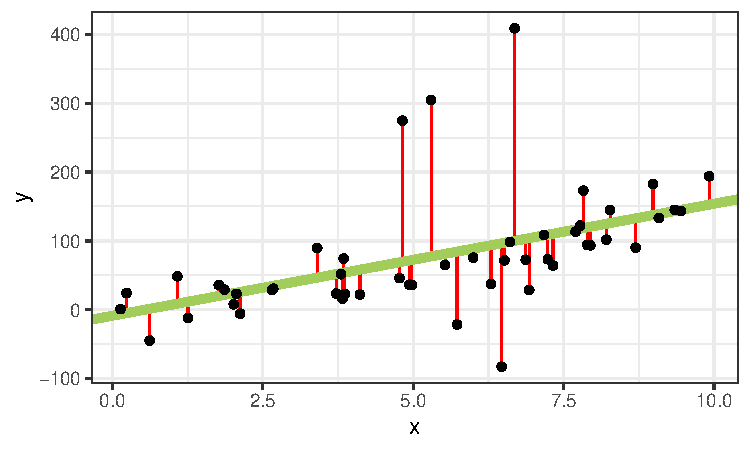
\includegraphics[width=\linewidth]{figure/lm_example.pdf}
\end{column}
\end{columns}
   
   %\vspace*{0.2cm} 
   \pause
    \textbf{Properties and assumptions} \citebutton{Faraway (2002), Ch. 7}{https://cran.r-project.org/doc/contrib/Faraway-PRA.pdf} \citebutton{Checking assumptions in R \& Python}{https://towardsdatascience.com/assumptions-of-linear-regression-fdb71ebeaa8b}
    \begin{itemize}[<+->]
    \item \textbf{Linear} relationship between features and target
    %Predictions are \textbf{linear} combination of features $\leadsto$ 
    %Model equation is additive and linear w.r.t. features% and identical across entire input space
    \item $\epsilon$ and $y \vert \xv$ are \textbf{normally} distributed with \textbf{constant variance} (homoscedastic)\\
    $\leadsto$ $\epsilon \sim N(0, \sigma^2) \; \Rightarrow \; (y \vert \xv) \sim N(\xv^\top \theta, \sigma^2)$\\
    $\leadsto$ if violated, inference-based metrics (e.g., p-values) are invalid
    %\item Error terms are assumed to have a \textbf{constant variance} over the entire feature space %(homoscedasticity)
    \item Independence of observations (e.g., no repeated measurements) %(e.g., no autocorrelated error terms)
    \item Independence of features $x_j$ with error term $\epsilon$
    \item No or little multicollinearity (i.e., no strong feature correlations)
    % free of measurement error assumption: https://indigo.uic.edu/articles/thesis/Measurement_Error_in_Generalized_Linear_Models/17025971/1/files/31488719.pdf
    % \item Note: For inference-based metrics (t-statistic, p-values, confidence intervals) to be valid, the error term needs to be normally distributed, i.e., $\epsilon \sim N(0, \sigma^2) \; \Rightarrow \; (y \vert x) \sim N(x^T \theta, \sigma^2)$\\
%$\leadsto$ Restricts use of LMs in practice as distribution of error is a prior assumption about data
        % \item Properties and assumptions:
        % \begin{itemize}
        %     \item linear
        %     \item normality assumption of the target % not true...
        %     \item homoscedastic (i.e., constant variance)
        %     \item independence of features
        %     \item fixed features (i.e., free of noise)
        %     \item no strong correlation of features
        % \end{itemize} 
    \end{itemize}

\end{frame}

%------------------------------------------------------------------
%------------------------------------------------------------------

\begin{frame}[c]{Linear Regression - Interpretation}

$$y = \theta_0 + \theta_1 x_1 + \theta_2 x_2 + \dots + \theta_p x_p + \epsilon = \xv^\top \theta + \epsilon$$

    Interpretation of weights (\textbf{feature effects}) depend on type of feature:
    \begin{itemize}[<+->]
        \item \textbf{Numerical $x_j$}: Increasing $x_j$ by one unit changes outcome by $\theta_j$, ceteris paribus (c.p.) \\ (\textit{ceteris paribus} means "everything else held constant".)
        \item \textbf{Binary $x_j$}: Weight $\theta_j$ is active or not (multiplication with 1 or 0) where 0 is reference category
    \end{itemize}

\begin{columns}[T, totalwidth = \linewidth]
\begin{column}{0.58\linewidth}
    \begin{itemize}
        \item<3-> %Categorical: One-hot-encoding of $L-1$ new features for $L$ categories (dummy encoding) \\
        \textbf{Categorical $x_j$ with $L$ categories}: Create $L-1$ one-hot-encoded features $x_{j,1}, \hdots, x_{j,L-1}$ (each having its own weight), left out category is reference ($\hat =$ dummy encoding)
        %$x_{j,l}, \forall l \in \{1, \hdots, L-1\}$ (with weight $\theta_{j,l}$), left out category is reference ($\hat =$ dummy encoding)
        \\
        $\leadsto$ Interpretation:
        Outcome changes by $\theta_{j,l}$ for category $l$ compared to reference cat.,  c.p.
        % (for any of the $L-1$ categories):
        %Predicted outcome changes for $l$-th category compared to the reference category by its weight $\theta_{j,l}$ c.p.
        %Predicted outcome changes for category $x_{j,l}$ compared to the reference category by $\theta_j$ c.p.
        \item<4> \textbf{Intercept $\theta_0$}: Expected outcome if all feature values are set to 0 %(baseline) %reflects expected features values if features were standardised (0-mean, 1-stdev)
        %\item Note: In case of higher order or interaction effects, weights cannot be interpreted in isolation
    \end{itemize}
\end{column}
\begin{column}{0.42\linewidth}
\begin{center}
        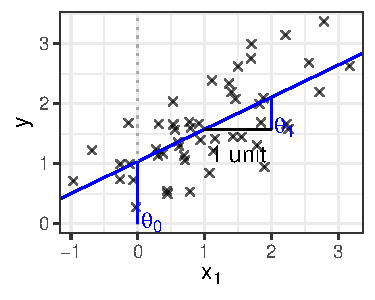
\includegraphics[width = 0.8\textwidth]{figure/reg_lm_plot_interpreted.pdf}\\
        % Bild aus I2ML: supervised-regression
        %figure/plot_lin_effect.pdf} \\
        %Boxplot of $\hat\theta_j x_j$-values (scale invariant)
        %$\leadsto$ Comparable feature contributions w.r.t. $\hat y$
    \end{center}
\end{column}
\end{columns}
    
\end{frame}

     
\begin{frame}[c]{Linear Regression - Interpretation}

$$y = \theta_0 + \theta_1 x_1 + \theta_2 x_2 + \dots + \theta_p x_p + \epsilon = \xv^\top \theta + \epsilon$$
    \textbf{Feature importance}:
    \begin{itemize}
        \item Absolute t-statistic value: $\hat\theta_j$ scaled with its standard error ($SE(\hat\theta_j)$ $\hat =$ reliability of the estimate) 
    $$|t_{\hat\theta_j}| = \left| \tfrac{\hat\theta_j}{SE(\hat\theta_j)} \right|$$
        \item High values indicate important (i.e. significant) features
    \end{itemize}
    \begin{center}
        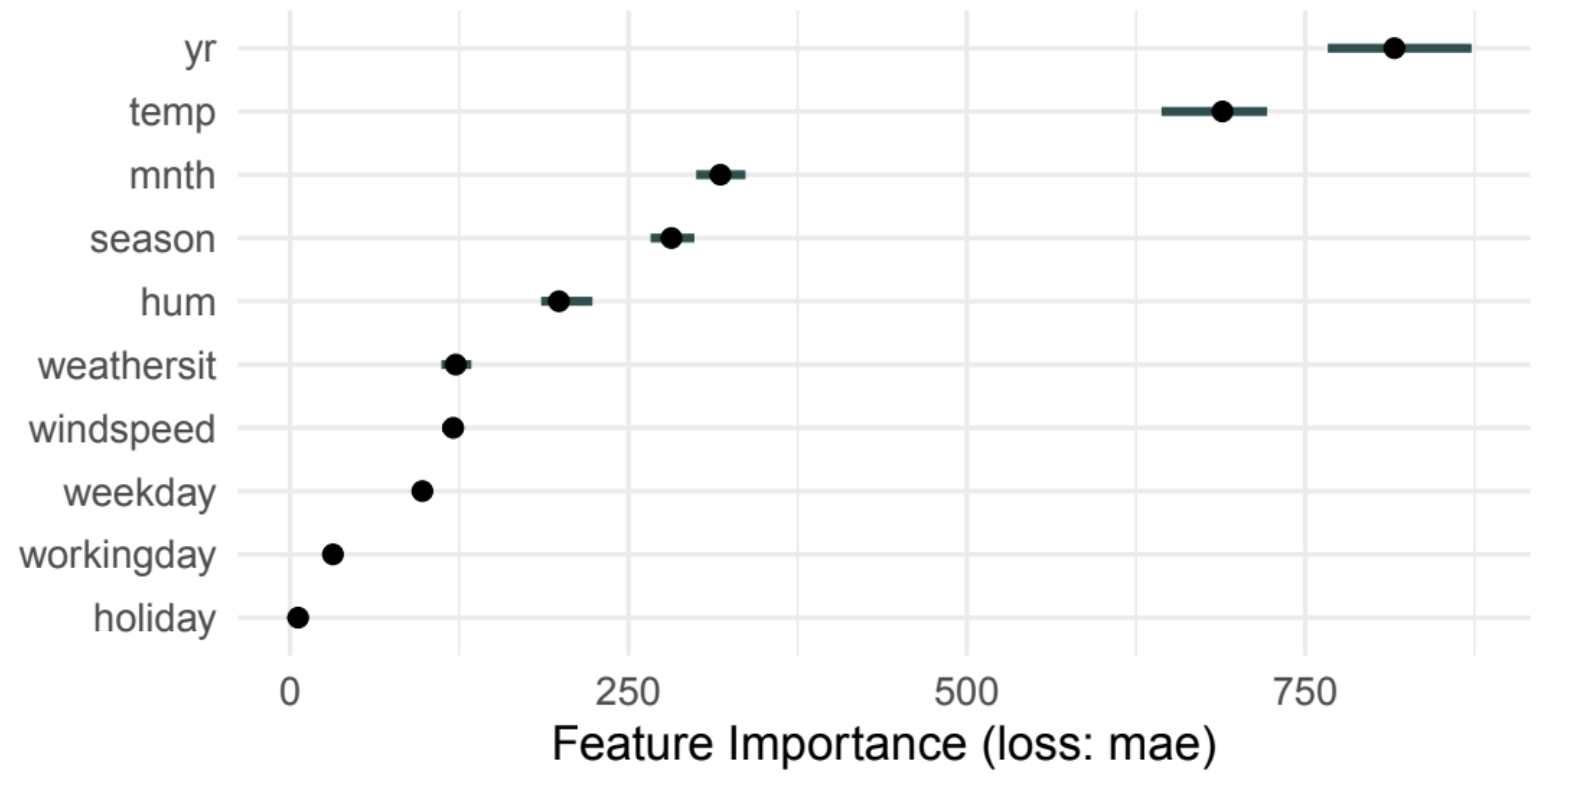
\includegraphics[width=0.4\textwidth]{../01_intro/figure/bike-sharing02.png}
    \end{center}
\end{frame}


\begin{frame}{Example: Linear Regression - Main Effects}

\textbf{Bike data}: predict number of rented bikes using 4 numeric and 1 categorical feature (season)

\medskip 

% \begin{footnotesize}
% $$
% \hat y = \hat \theta_0 + \hat \theta_1 \mathds{1}_{(seas = SPRING)} + \hat \theta_2 \mathds{1}_{(seas = SUMMER)} + \hat \theta_3 \mathds{1}_{(seas = FALL)} + \hat \theta_4 temp + \hat \theta_5 hum + \hat \theta_6 windspeed + \hat \theta_7 days\_since\_2011
% $$
% \end{footnotesize}
\begin{columns}[T, totalwidth=\linewidth]
\begin{column}{0.52\textwidth}
%\vspace*{-0.3cm}
\begin{align*}
\hat y = 
& \hat \theta_0 + 
\hat \theta_1 \mathds{1}_{x_{season} = SPRING} +
\hat \theta_2 \mathds{1}_{x_{season} = SUMMER} +\\
& 
\hat \theta_3 \mathds{1}_{x_{season} = FALL} + 
\hat \theta_4 x_{temp} + 
\hat \theta_5 x_{hum} + \\
& 
\hat \theta_6 x_{windspeed} + 
\hat \theta_7 x_{days\_since\_2011}
\end{align*}
\end{column}
\begin{column}{0.47\textwidth}
  \centering
\begin{scriptsize}
%\begin{overlayarea}{\textwidth}{\textheight}
%\begin{table}[ht]
\only<2>{\def\firstrowcolor{\rowcolor{lightgray}}}
\only<3>{\def\secondrowcolor{\rowcolor{lightgray}}}
\only<4>{\def\thirdrowcolor{\rowcolor{lightgray}}}
\begin{tabular}{rrrrr}
  \hline
 & Weights & SE & t-stat. & p-val. \\
 \hline
\firstrowcolor (Intercept) & 3229.3 & 220.6 & 14.6 & 0.00 \\ 
\secondrowcolor seasonSPRING & 862.0 & 129.0 & 6.7 & 0.00 \\ 
  seasonSUMMER & 41.6 & 170.2 & 0.2 & 0.81 \\ 
  seasonFALL & 390.1 & 116.6 & 3.3 & 0.00 \\ 
\thirdrowcolor temp & 120.5 & 7.3 & 16.5 & 0.00 \\ 
  hum & -31.1 & 2.6 & -12.1 & 0.00 \\ 
  windspeed & -56.9 & 7.1 & -8.0 & 0.00 \\ 
  days\_since\_2011 & 4.9 & 0.2 & 26.9 & 0.00 \\
   \hline
\end{tabular}
%\end{table}
%\end{overlayarea}
\end{scriptsize}
\end{column}
\end{columns}
%\vspace*{-0.3cm}
\pause

\lz
%\begin{columns}[T, totalwidth=\linewidth]
%\begin{column}<5>{0.46\textwidth}
%\textbf{Vis.}: Boxplot of $\hat\theta_j x_j$-values (scale invariant)\\
%weights multiplied by actual feature value (better comparable due to different scales)
%$\leadsto$ Comparable feature contributions w.r.t. $\hat y$

%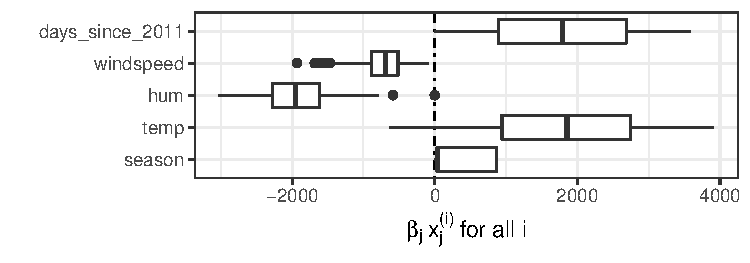
\includegraphics[width = \textwidth]{figure/plot_lin_effect.pdf}
%   \begin{center}
%   % Effect of $i$-th observation $= \theta_j x_j^{(i)}$\\

%     %$\leadsto$ Better comparability due to different scales
%   \end{center}
%\pause
%\verbatiminput{figure/lm_output.txt}
%\end{column}\hfill
%\begin{column}{0.54\textwidth}  %%<--- here

\begin{itemize}[<+->]
    \item \textbf{Interpretation intercept}:
    If all feature values are 0 (and season is \code{WINTER} $\hat =$ reference cat.), the expected number of bike rentals is $\hat\theta_0 = 3229.3$
    \item \textbf{Interpretation categorical}: Rentals in \code{SPRING} are by $\hat\theta_1 = 862$ higher than in \code{WINTER}, c.p.
    \item \textbf{Interpretation numerical}: Rentals increase by $\hat\theta_4 = 120.5$ if \code{temp} increases by 1 $^{\circ}$C, c.p.
    %If the temperature increases by 1 order Celsius, the number of bike rentals increases by 120.5 c.p.

\end{itemize}
%\end{column}
%\end{columns}
\end{frame}


%------------------------------------------------------------------
%------------------------------------------------------------------

\begin{frame}{Linear Regression - Interaction and High-order Effects}

$$y = \theta_0 + \theta_1 x_1 + \theta_2 x_2 + \dots + \theta_p x_p + \epsilon$$

Equation above can be extended (polynomial regression) by including

\begin{itemize}
\item \textbf{high-order effects} which have their own weights\\
$\leadsto$ e.g., quadratic effect: $\theta_{x_j^2} \cdot x_j^2$
\item \textbf{interaction effects} as the product of multiple features\\
$\leadsto$ e.g., 2-way interaction: $\theta_{x_i, x_j} \cdot x_i \cdot x_j$
\end{itemize}
\pause
Implications of including high-order and interaction effects: 
\begin{itemize}
    \item Both make the model more flexible but also less interpretable\\
    $\leadsto$ More weights to interpret
    \item Both need to be specified manually (inconvenient and sometimes infeasible)\\
    $\leadsto$ Other ML models learn them often automatically
    \item Marginal effect of a feature cannot be interpreted by single weights anymore\\
$\leadsto$ Feature $x_j$ occurs multiple times (with different weights) in equation
\end{itemize}

%Weights cannot be interpreted in isolation as before
% $$y = \theta_0 + \theta_1 x_1 + \theta_2 x_2 + \dots + \theta_p x_p + \epsilon$$

% \begin{itemize}
% \item Results in polynomial regression 
% \item Weights cannot be interpreted in isolation as before
% \end{itemize}
\end{frame}

% \begin{frame}{Linear and Polynomial Regression}

% \begin{align*}
% \mathbb{E}_Y(Y \vert X) &= \theta_0 + \theta_1 x_1 + \dots + \theta_p x_p + \epsilon \\
%  &= X^T\theta + \mathcal{E}
% \end{align*}

% \begin{itemize}
% \itemsep1em
% \item Model equation is identical across the entire feature space.
% %\item The predictive power of LMs is determined by specifying the correct model structure.
% \item Polynomial regression extends the LM by non-linear effects.
% %A polynomial regression model is an extension of the LM that includes higher order terms or interactions.
% %This enables us to model non-linear data while making use of the entire arsenal of LM functionality.
% \item We can exactly determine feature effects (e.g., beta coefficients, effect plots) and importance scores (e.g., p-values, t-statistics).
% %By knowing the model equation, we can exactly determine feature effects (e.g., beta coefficients, effect plots) and importance scores (e.g., p-values, t-statistics).
% \item For higher order effects or interactions, beta coefficients cannot be interpreted in isolation.
% \item Note: For inference-based metrics (p-values, confidence intervals) to be valid, error term needs to be normally distributed with zero mean, i.e., $\epsilon \sim N(0, \sigma^2) \; \Rightarrow \; (y \vert x) \sim N(x^T \theta, \sigma^2)$.\\
% $\leadsto$ Restricts use of LMs in practice as distribution of error is a prior assumption about data.
% \end{itemize}
% \end{frame}

\begin{frame}{Example: Linear Regression - Interaction Effect}
\textbf{Example}: Interaction between \code{temp} and \code{season} will affect marginal effect of \code{temp}% with (right) and without (left) interaction.
\begin{columns}[T, totalwidth=\linewidth]
\begin{column}{0.65\linewidth}
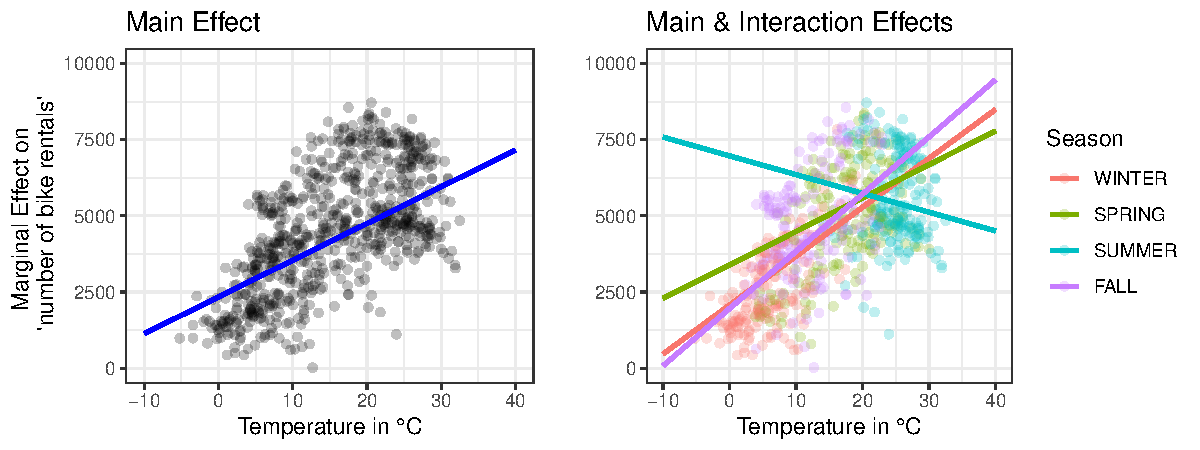
\includegraphics[width = \textwidth]{figure/lm_main_vs_interaction_effects.pdf}
\end{column}
\begin{column}{0.35\linewidth}
\begin{scriptsize}
%\begin{table}[ht]
\only<2->{\def\firstrowcolor{\rowcolor{lightgray}}}
\only<3>{\def\secondrowcolor{\rowcolor{lightgray}}}
\only<4>{\def\thirdrowcolor{\rowcolor{lightgray}}}
\only<5>{\def\fourthrowcolor{\rowcolor{lightgray}}}
\centering
\begin{tabular}{rr}
  \hline
 & Weights \\ 
  \hline
(Intercept) & 3453.9 \\ 
  seasonSPRING & 1317.0 \\ 
  seasonSUMMER & 4894.1 \\ 
  seasonFALL & -114.2 \\ 
  \firstrowcolor temp & 160.5 \\ 
  hum & -37.6 \\ 
  windspeed & -61.9 \\ 
  days\_since\_2011 & 4.9 \\
  \hline
  \secondrowcolor seasonSPRING:temp & -50.7 \\ 
  \thirdrowcolor seasonSUMMER:temp & -222.0 \\ 
  \fourthrowcolor seasonFALL:temp & 27.2 \\ 
   \hline
\end{tabular}
%\end{table}
\end{scriptsize}
\end{column}
\end{columns}
\vfill
\pause
\begin{columns}[T, totalwidth=\linewidth]
\begin{column}{0.6\linewidth}
\textbf{Interpretation}: If \code{temp} increases by 1 $^{\circ}$C, bike rentals
\begin{itemize}[<+->]
    \item increase by 160.5 in \code{WINTER} (reference)
    \item increase by 109.8 (= 160.5 - 50.7) in \code{SPRING}
    \item decrease by -61.5 (= 160.5 - 222) in \code{SUMMER}
    \item increase by 187.7 (= 160.5 + 27.2) in \code{FALL}
\end{itemize} %\\\vspace*{0.2cm}
\end{column}
\begin{column}{0.4\linewidth}
% \lz
% \only<6>{\textbf{Note:}
% Temperature values (on x-axis) depend on \code{season}\\
% $\leadsto$ not acknowledged by LM\\
% $\leadsto$ misleading interpretation due to extrapolation in regions with few points (e.g. low \code{temp} in \code{SUMMER})
% }
\end{column}
\end{columns}
%Value ranges of temperature differ depending on the season $\leadsto$ not acknowledged by LM
\end{frame}


\begin{frame}{Example: Linear Regression - Quadratic Effect}
\textbf{Example}: Adding quadratic effect for \code{temp} \only<2>{(left) and an interaction with \code{season} (right)}
\begin{columns}[T, totalwidth=\linewidth]
\begin{column}{0.65\linewidth}
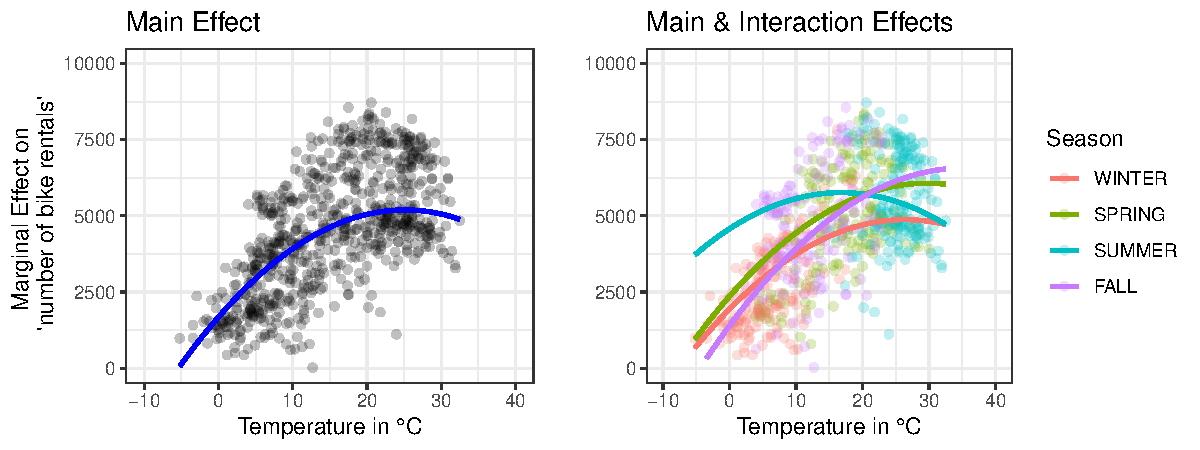
\includegraphics[width=0.5\textwidth, trim=0cm 0.1cm 10.4cm 0cm, clip]{figure/poly_main_vs_interaction_effects.pdf}\invisible<1>{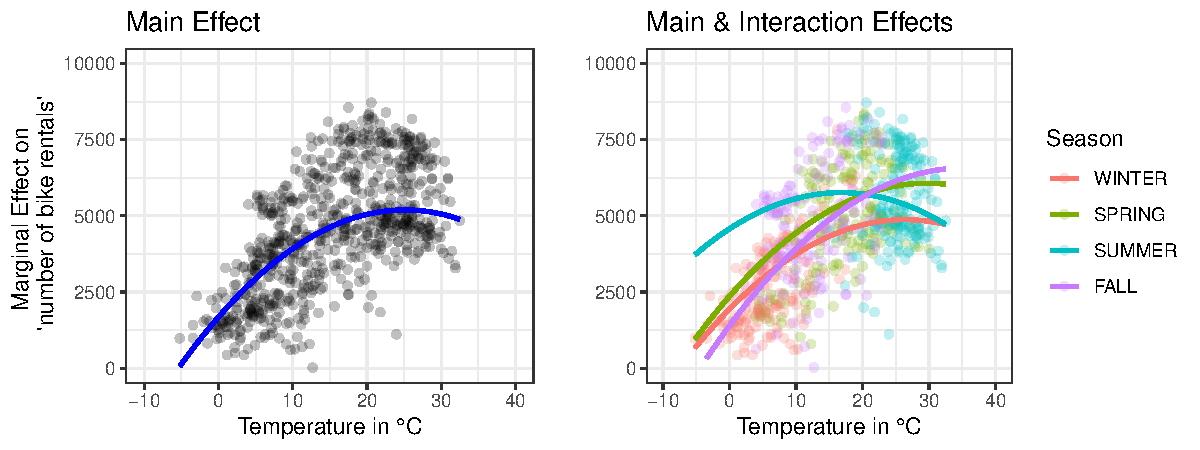
\includegraphics[width=0.5\textwidth, trim=10cm 0.1cm 0.4cm 0cm, clip]{figure/poly_main_vs_interaction_effects.pdf}}
%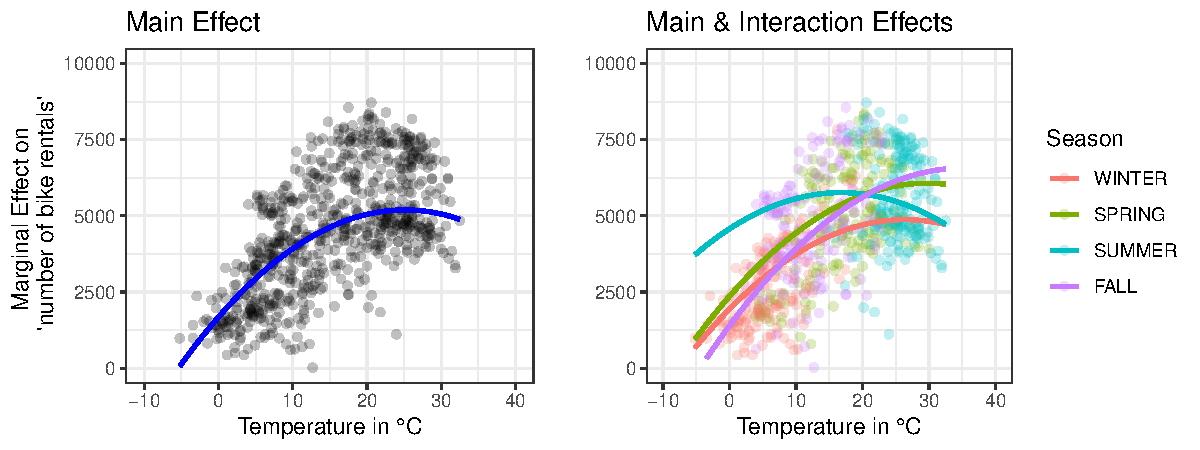
\includegraphics[width = \textwidth]{figure/poly_main_vs_interaction_effects.pdf}
%\begin{columns}
%\begin{center}
%\adjincludegraphics[width=\textwidth, trim={0 0 {.55\width} 0}, clip]{figure/poly_main_vs_interaction_effects.pdf}

\textbf{Interpretation}: Not linear anymore!
\begin{itemize}
    \only<1>{\item[$\leadsto$] \code{temp} depends on two weights: $ 280.2 \cdot x_{temp} -  5.6 \cdot x_{temp}^2$}
    \item<2>[$\leadsto$] \code{temp} depends on multiple weights due to \code{season}:\\
    $\leadsto$ \code{WINTER}: ${\color{winter}39.1} \cdot x_{temp} + {\color{winter}8.6} \cdot x_{temp}^2$ \\
    $\leadsto$ \code{SPRING}: 
    $({\color{winter}39.1} {\color{spring}+407.4}) \cdot x_{temp} + ({\color{winter}8.6} {\color{spring} - 18.7}) \cdot x_{temp}^2$ \\
    $\leadsto$ \code{SUMMER}: $({\color{winter}39.1}  {\color{summer}+801.1}) \cdot x_{temp} + ({\color{winter}8.6} {\color{summer} - 27.2}) \cdot x_{temp}^2$  \\
    $\leadsto$ \code{FALL}: $({\color{winter}39.1}  {\color{fall}+217.4}) \cdot x_{temp} + ({\color{winter}8.6} {\color{fall} - 11.3}) \cdot x_{temp}^2$ 
    % \item<2>[$\leadsto$] High-order and interaction effects make the model more flexible but also less interpretable (more weights)
    % \item<2>[$\leadsto$] High-order and interaction effects need to be specified manually (inconvenient) - ML models do this automatically
\end{itemize}

\end{column}
\begin{column}{0.35\linewidth}
%\hfill
\begin{scriptsize}
% \begin{table}[ht]
% %\centering

\def\firstrowcolor{\rowcolor{lightgray}}%
\def\secondrowcolor{\rowcolor{spring}}%
\def\thirdrowcolor{\rowcolor{summer}}%
\def\fourthrowcolor{\rowcolor{fall}}%

\only<1>{%
\begin{tabular}{rr}
  \hline
 & Weights \\ 
  \hline
(Intercept) & 3094.1 \\ 
  seasonSPRING & 619.2 \\ 
  seasonSUMMER & 284.6 \\ 
  seasonFALL & 123.1 \\ 
  hum & -36.4 \\ 
  windspeed & -65.7 \\ 
  days\_since\_2011 & 4.7 \\ 
  \firstrowcolor temp & 280.2 \\ 
  \firstrowcolor temp$^2$ & -5.6 \\ 
  \hline
\end{tabular}%
}
% \end{table}
\only<2>{%
\def\firstrowcolor{\rowcolor{winter}}%
\begin{tabular}{rr}
  \hline
 & Weights \\ 
  \hline
(Intercept) & 3802.1 \\ 
  seasonSPRING & -1345.1 \\ 
  seasonSUMMER & -6006.3 \\ 
  seasonFALL & -681.4 \\ 
  hum & -38.9 \\ 
  windspeed & -64.1 \\ 
  days\_since\_2011 & 4.8 \\ 
 \firstrowcolor temp & 39.1 \\ 
 \firstrowcolor temp$^2$ & 8.6 \\ 
  \hline
  \hline
  \secondrowcolor seasonSPRING:temp & 407.4 \\ 
 \secondrowcolor seasonSPRING:temp$^2$ & -18.7 \\ 
  \thirdrowcolor seasonSUMMER:temp & 801.1 \\ 
 \thirdrowcolor seasonSUMMER:temp$^2$ & -27.2 \\ 
  \fourthrowcolor seasonFALL:temp & 217.4 \\ 
 \fourthrowcolor seasonFALL:temp$^2$ & -11.3 \\ 
   \hline
\end{tabular}%
}%
%Table: Weights for main effect model
\end{scriptsize}
%\end{center}
\end{column}
\end{columns}
\end{frame}


\begin{frame}{Regularization via LASSO \citebutton{Tibshirani (1996)}{https://doi.org/10.1111/j.2517-6161.1996.tb02080.x}}
% \begin{itemize}
%     \item LASSO adds an $L_1$-norm penalization term ($\lambda||\theta||_1$) to the least squares optimization problem%\\
%     % $\leadsto$ Shrinks some feature weights to zero (feature selection)\\
%     % $\leadsto$ Sparser models (with fewer features) are more interpretable
%     % %Aim: Feature selection (sparsity) and regularization of feature weights
%     % \item Penalization parameter $\lambda$ must be chosen (e.g., by CV) %or depending on the number of features to keep
% \end{itemize}

\begin{columns}[T, totalwidth=\linewidth]
\begin{column}{0.65\textwidth}
\begin{itemize}
    \item LASSO adds an $L_1$-norm penalization term ($\lambda||\theta||_1$) \\%to the least squares optimization problem\\
    $\leadsto$ Shrinks some feature weights to zero (feature selection)\\
    $\leadsto$ Sparser models (fewer features): more interpretable
    %Aim: Feature selection (sparsity) and regularization of feature weights
    \item Penalization parameter $\lambda$ must be chosen (e.g., by CV) %or depending on the number of features to keep
\end{itemize}
$$
min_{\theta} \bigg(\underbrace{\frac{1}{n} \sum_{i=1}^{n} (y^{(i)} - {\xi}^{\top} \theta)^2}_\text{Least square estimate for LM} + \lambda||\theta||_1\bigg) 
$$
%\vspace*{0.2cm}\\
%\vspace*{-0.4cm}
%\pause
\only<2->{
\textbf{Example} (interpretation of weights analogous to LM):
\begin{itemize}
    \item LASSO with main effects and interaction \code{temp} with \code{season}
    \item $\lambda$ is chosen such that 6 features are selected (not zero)
    \item For categorical features, LASSO shrinks weights of single categories separately (due to dummy encoding)\\
    %only weights of single categories are set to zero (due to dummy encoding) not the whole feature\\
    $\leadsto$ No feature selection of whole categorical features\\
    %May be problematic for categorical features as only weights of single categories are set to zero (due to dummy encoding) instead of the whole categorical feature\\ %, polynomials and interactions
    $\leadsto$ Solution: group LASSO \citebutton{Yuan and Lin (2006)}{https://doi.org/10.1111/j.1467-9868.2005.00532.x}
\end{itemize}}
\end{column}
\begin{column}{0.35\textwidth}
\centerline{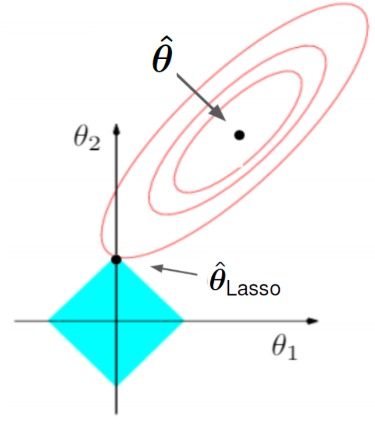
\includegraphics[width=0.5\textwidth]{figure/l1_hat.png}} 
%\lz\lz
\scriptsize
\vspace{0.1cm}
%\begin{table}[b]
\only<2->{
\centering
\begin{tabular}{rr}
  \hline
 & Weights \\ 
  \hline
(Intercept) & 3135.2 \\ 
  seasonSPRING & 767.4 \\ 
  seasonSUMMER & 0.0 \\ 
  seasonFALL & 0.0 \\ 
  temp & 116.7 \\ 
  hum & -28.9 \\ 
  windspeed & -50.5 \\ 
  days\_since\_2011 & 4.8 \\ 
  \hline
  seasonSPRING:temp & 0.0 \\ 
  seasonSUMMER:temp & 0.0 \\ 
  seasonFALL:temp & 30.2 \\ 
   \hline
\end{tabular}
%\end{table}
% \begin{table}[ht]
% \centering
% \begin{tabular}{rr}
%   \hline
%  & Weights \\ 
%   \hline
% (Intercept) & 2665.50 \\ 
%   seasonSPRING & 489.34 \\ 
%   seasonSUMMER & 0.00 \\ 
%   seasonFALL & 0.00 \\ 
%   hum & -19.44 \\ 
%   windspeed & -35.54 \\ 
%   days\_since\_2011 & 4.71 \\ 
%   poly(temp, 2)1 & 109.25 \\ 
%   poly(temp, 2)2 & 0.00 \\ 
%   \hline
% \end{tabular}
% \end{table}
}
\end{column}
\end{columns}

\end{frame}
\endlecture
\end{document}